
\chapter{Neutrino masses}

\section{Standard model particle content}

\begin{frame}[fragile,allowframebreaks]
In the following discussion we use the following doublets
\begin{align}
  H=&
  \begin{pmatrix}
    H^+\\
    H^0
  \end{pmatrix},&
  L_i=&
  \begin{pmatrix}
    \nu_{Li}\\
    e_{Li}^{-}
  \end{pmatrix}.
\end{align}
corresponding to the Higgs doublet and the lepton doublets respectively.
\end{frame}

\section{Weinberg operator}

\begin{frame}[fragile,allowframebreaks]
See Weinberg,  PRL43(1979)1566:
 \begin{align*}
   \mathcal{L}
   =&\frac{y_{ij}}{\Lambda} L_i\cdot H L_j\cdot H+\text{h.c}\nonumber\\
   =&\frac{y_{ij}}{\Lambda}\epsilon_{ab}\epsilon_{cd} L^a_i H^b L^c_j H^d+\text{h.c}\,.
 \end{align*}
\end{frame}
where $y_{ij}$ are adimensional couplings and $\Lambda$ some high-scale.
The treatment in four notation component is given in Sec.~\ref{sec:4weinberg-operator}.

For a discussion around this operator see for example~\url{http://bit.ly/neutrinoreview}.

This operator breaks Lepton number ($L$) by two units, where the $L=-1$ and $0$ for $L_i$ and $H$ respectively.
In the same paradigm of the standard model, it is expected that the mass terms associated with the $\Lambda$ scale would be related to the spontaneous breaking of some symmetry. 



\section{Type-I seesaw}

To keep the paradigm of the standard model where the masses of the fundamental fields must be generated from the spontaneous breaking of some symmetry, we assume that at some scale $\Lambda$ the lepton number is still preserved even after the introduction of right-handed neutrinos
\begin{frame}[fragile,allowframebreaks]
\begin{align}
  \mathcal{L}_{\nu}=y_{i} \left( N_R \right)^{\dagger} L_i\cdot  H   
  +\tfrac{1}{2} h_R\, N_R  N_R S + \text{h.c}\,.
\end{align}
where $y_i$ and $h_R$ are adimensional couplings, while $S$ is an scalar singlet which can acquire a vacuum expectation value $\langle S \rangle$, such that the right handed neutrino can acquire a Majorana mass
\begin{align}
  M_R=h_R \langle S \rangle\,.
\end{align}
The assignment of $L$ is given in Table~\ref{tab:Lassign}
\begin{table}
  \centering
  \begin{tabular}{c|c}
    Field& $\operatorname{U}(1)_L$\\ \hline
    $L_i$& $-1$ \\
    $H$& $\phantom{-}0$ \\
    $N_{R}$& $-1$ \\
    $S$&$+2$
  \end{tabular}
  \caption{Lepton number flux in green }
  \label{tab:Lassign}
\end{table}

We can build the diagram displayed in fig.~\ref{fig:lnv}, where the arrows indicate the flux of lepton number. 

\begin{figure}
  \centering
  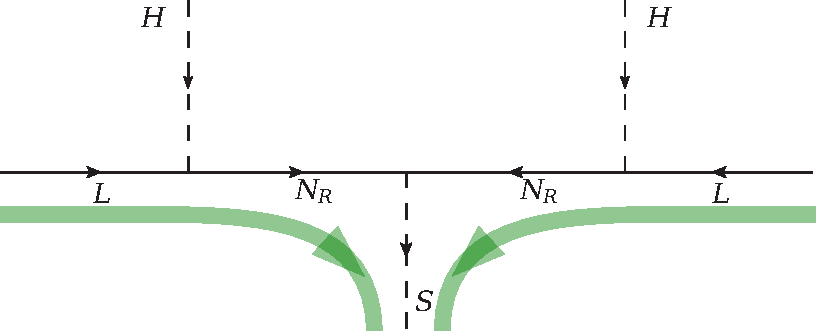
\includegraphics[scale=0.6]{seesawm}
  \caption{Seesaw mechanism}
  \label{fig:lnv}
\end{figure}

\end{frame}
After the spontaneous symmetry breaking,
\begin{frame}[fragile,allowframebreaks]
if we assume to have just one right-handed neutrino $N_R$ 
\begin{align}
  \label{eq:lnv}
  \mathcal{L}_{\nu}=y_{i} \left( N_R \right)^{\dagger} L_i\cdot  H   
  +\tfrac{1}{2} M_R\, N_R  N_R + \text{h.c}\,.
\end{align}
To track down the relevant term beyond the standard model, it is convenient to reassign $L$ such that the resulting lepton number violating terms involve some of standard model fields. In fact, by reassigning $L=0$ to $N_R$, it turns out that the only lepton number violating terms are the ones involving the Yukawa coupling $y_i$ in eq~\eqref{eq:lnv}.
\end{frame}
\begin{frame}[fragile,allowframebreaks]
In addition to the previous Majorana mass contribution $M_R$, after the spontaneous symmetry breaking the neutral states $\nu_{Li}$ and $N_R$  acquire a Dirac mass contribution

\begin{align}
  \mathcal{L}_{\nu}\supset & M_D^{i} \left( \nu_{Li} \right)^{\dagger} N_R +\frac{1}{2} M_R N_R N_R +\text{h.c} \nonumber\\
  =&  \frac{1}{2}M_D^{i} \left( \nu_{Li} \right)^{\dagger} N_R
     +\frac{1}{2}M_D^{i} N_R\left( \nu_{Li} \right)^{\dagger} +\frac{1}{2} M_R N_R N_R +\text{h.c} \nonumber\\
  =&\frac{1}{2}\begin{pmatrix} \left( \boldsymbol{\nu}_{L} \right)^{\dagger}  & N_R  \end{pmatrix}
 \begin{pmatrix}
   \mathbf{0}_{3 \times 3} &            \boldsymbol{M}_D \\
   \boldsymbol{M}_D^{\operatorname{T}} & M_R \\
 \end{pmatrix}
\begin{pmatrix} \left( \boldsymbol{\nu}_{L} \right)^{\dagger}  \\
    N_R  \end{pmatrix}+\text{h.c} \nonumber\\
  \equiv&\frac{1}{2} \boldsymbol{\chi}^{\operatorname{T}} \boldsymbol{M_{\chi}} \boldsymbol{\chi}+\text{h.c}\,,
\end{align}
\end{frame}
\begin{frame}[fragile,allowframebreaks]
where the Dirac neutrino mass vector $\boldsymbol{M}_D$ has components
\begin{align}
  M_D^i=\frac{y^i v}{\sqrt{2}}\,,
\end{align}
$\left( \boldsymbol{\nu}_{L} \right)^{\dagger\operatorname{T}}=
\begin{pmatrix}\nu_{L1} & \nu_{L2} & \nu_{L3} \end{pmatrix}^{\operatorname{T}}$, $\boldsymbol{\chi}^{\operatorname{T}}=\begin{pmatrix} \left( \boldsymbol{\nu}_L \right)^{\dagger}  & N_R  \end{pmatrix}^{\operatorname{T}}$, and
\begin{align}
  \boldsymbol{M_{\chi}}=& \begin{pmatrix}
   \mathbf{0}_{3 \times 3} &            \boldsymbol{M}_D \\
   \boldsymbol{M}_D^{\operatorname{T}} & M_R \\
 \end{pmatrix}
\end{align}
which has eigenvalues
\begin{align}
{  \boldsymbol{M_{\chi}}}_\mp=&\frac{1}{2} \left[ M_R \mp \left( M_R^2 + 4   \boldsymbol{M}_D   \boldsymbol{M}_D^{\operatorname{T}}  \right)^{1/2} \right] \nonumber\\
  =&\frac{1}{2} M_R\left[ 1 \mp  \left( 1 + 4   \boldsymbol{M}_D M_R^{-2}   \boldsymbol{M}_D ^{\operatorname{T}}  \right)^{1/2} \right].
\end{align}
When $M_R^2 \gg \boldsymbol{M}_D  \boldsymbol{M}_D ^{\operatorname{T}} $
\begin{align}
  { \boldsymbol{M_{\chi}}}_\mp\approx &\frac{1}{2} M_R\left[ 1 \mp  \left( 1 +   2 \boldsymbol{M}_D M_R^{-2}   \boldsymbol{M}_D^{\operatorname{T}}  \right)
   \right]
\end{align}
\end{frame}
\begin{frame}[fragile,allowframebreaks]
Therefore
\begin{align}
 \boldsymbol{\mathcal{M}}_{\nu}\to {M_{\chi^-} }\approx&-   \boldsymbol{M}_D M_R^{-1}   \boldsymbol{M}_D^{\operatorname{T}}  \nonumber\\
 M_{\chi^+} \approx&    M_R\,.
\end{align}

The effective neutrino mass matrix, $\boldsymbol{\mathcal{M}}_{\nu}$,  in this case   is just a rank one matrix
\begin{align}
  \boldsymbol{\mathcal{M}}_{\nu}\to&- \boldsymbol{M}_D M_R^{-1} \boldsymbol{M}_D^{\operatorname{T}}\nonumber\\
  \left( {\mathcal{M}}_{\nu} \right)_{ij}\approx&- M_D^i M_R^{-1} M_D^{j}\,.
\end{align}
\end{frame}
It is possible to write the final result in terms of a Majorana fermion defined from the Weyl spinors in the diagonal by blocks basis, denoted with a zero superindex be
low.
\begin{frame}[fragile,allowframebreaks]
We have
\begin{align}
  \boldsymbol{\nu}=&
  \begin{pmatrix}
    \boldsymbol{\nu}_L^0\\
    \left( \boldsymbol{\nu}_L^0 \right)^{\dagger}\\
  \end{pmatrix},&       \boldsymbol{m}_{\nu}=& \begin{pmatrix}
                                      \boldsymbol{\mathcal{M}}_{\nu} & \boldsymbol{0} \\
                                      \boldsymbol{0} & \boldsymbol{\mathcal{M}}_{\nu}  \\
                                    \end{pmatrix}.
\end{align}
Therefore
\begin{align}
  \mathcal{L}_{\nu}\supset &\, \tfrac{1}{2}\,\overline{\boldsymbol{\nu}^c}\, \boldsymbol{m}_{\nu} \boldsymbol{\nu}   \nonumber\\
=& \cdots \nonumber\\
=&\tfrac{1}{2}\,\boldsymbol{\nu}_L^{0}\, \boldsymbol{\mathcal{M}}_{\nu}\,   \boldsymbol{\nu}_L^{0} +\text{h.c}\,.
\end{align}
\end{frame}

Note that Abelian Lepton number is not longer a conserved symmetry of the Lagrangian. For example by assigning Lepton $-1$ for $N_R$, the Majorana term $N_R N_R$ violates Lepton number by two units. However we can identify a remnant $Z_{2}$ symmetry under which the Leptons are odd and all the other SM particles are even, including the Higgs doublet. This symmetry is called Lepton parity.


\section{Dirac operator}

If neutrinos are Dirac particles, the Standard Model (SM) particle content must be extended with right-handed neutrinos, and some symmetry must be imposed to prevent their Majorana mass terms.
\begin{frame}[fragile,allowframebreaks]
At least a $Z_3$ symmetry is required to forbid both the tree-level Yukawa terms  and Majorana mass terms
\begin{align}
  \label{eq:tld}
%  \mathcal{L}_{\nu}=&\,y_D\left( \nu_R \right)^{\dagger} \epsilon_{ab}L^a H^b+\text{h.c.} \nonumber\\
  \mathcal{L}_{\nu}=&\,y^D_{\alpha i}\left( \nu_{R\alpha} \right)^{\dagger} L_i\cdot H +\frac{1}{2}m_R \nu_R \nu_R+\text{h.c}\,,
\end{align}
\end{frame}
with $L_i\cdot H=\epsilon_{ab}L^a_i H^b$, where $L_i$ are the lepton doublets, $H$ is the
SM Higgs doublet with hypercharge $Y=1$, and $y_D$ is the matrix of neutrino Yukawa couplings.  
A possible assignment to forbid only the Majorana mass term is obtained if the SM fields that transform
non-trivially under $Z_3$ as: $L\sim \omega$,
$\left( e_R \right)^{\dagger} \sim \omega^2$ and
$\left( \nu_R \right)^{\dagger} \sim \omega^2$, with $\omega^3=1$.
\begin{frame}[fragile,allowframebreaks]
At this level, the neutrino mass problem is not longer a
phenomenological issue but a theoretical one, in which it is necessary
to explain the smallness of the Yukawa couplings in $y_D$, which must be  of order
$10^{-11}$.

To do so, we assume that the symmetry allows for the 5-dimensional operator with total lepton number conservation~\cite{Gu:2006dc}
\begin{align}
  \label{eq:blop}
  \mathcal{L}_5=
  \frac{y_{\alpha i}}{\Lambda} \left( \nu_{R\alpha} \right)^\dagger  L_i\cdot H\, S + 
\text{h.c.}\,,
\end{align}
\end{frame}
where $y_{\alpha i}$ are adimensional couplings and $\Lambda$ is the new physics scale.
To be compatible with  neutrino
oscillation data \cite{deSalas:2017kay}, $y$ should be at least of order $2\times 3$.  



\section{Dirac Type-I seesaw  }
\begin{frame}[fragile,allowframebreaks]
We need to assume the existence of a heavy Dirac fermion, $F=
\begin{pmatrix}
  F_L & F_R
\end{pmatrix}^{\operatorname{T}}$, where $F_{LR}$ are Weyl fermions, and one real scalar singlet $S$. The most general Lagrangian is~\cite{Roncadelli:1983ty}
\begin{align}
  \mathcal{L}_{\nu}=y_i \left(  F_R \right)^{\dagger}L_i\cdot H  
  + M_F\, \left( F_L \right)^{\dagger}  F_R + h_i \left( F_L \right)^{\dagger} S \nu_{Ri}+   \text{h.c}\,.
\end{align}

The assignment of $L$ is given in Table~\ref{tab:Lassignd}
\begin{table}
  \centering
  \begin{tabular}{c|c}
    Field& $\operatorname{U}(1)_L$\\ \hline
    $L_i$& $-1$ \\
    $H$& $\phantom{-}0$ \\
    $\nu_{R}$& $-4$ \\
    $S$&$+3$
  \end{tabular}
  \caption{Lepton number flux in green }
  \label{tab:Lassignd}
\end{table}

We can build the diagram displayed in fig.~\ref{fig:cln}, where the arrows indicate the flux of lepton number. 

\begin{figure}
  \centering
  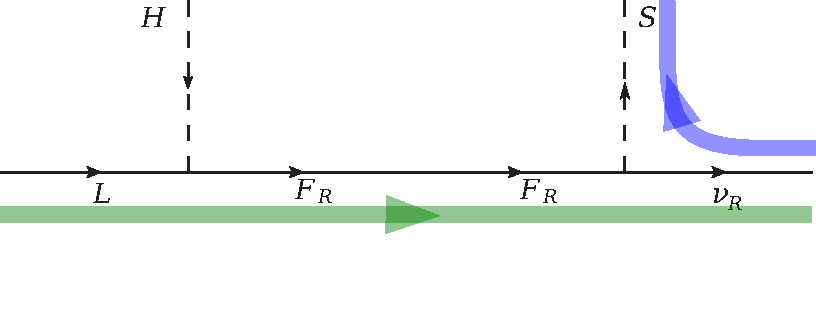
\includegraphics[scale=0.6]{seesawd}
  \caption{Seesaw mechanism}
  \label{fig:cln}
\end{figure}


In addition to the previous Dirac mass contribution $M_F$, after the full spontaneous symmetry  breaking the neutral states $\nu_{Li}$ and $\nu_{Ri}$  acquire a Dirac mass contributions $M_{Di}$ and $M_{Si}$ respectively
\begin{align}
  \mathcal{L}_{\nu}\supset & M_{Di} \left( \nu_{Li} \right)^{\dagger}_i  F_R 
  + M_F\, \left( F_L \right)^{\dagger}  F_R + M_{Si} \left( F_L \right)^{\dagger}  \nu_{Ri}+   \text{h.c}\,. \nonumber\\
  =&\begin{pmatrix} \left( \boldsymbol{\nu}_{L} \right)^\dagger  & \left( F_L \right)^{\dagger}  \end{pmatrix}
 \begin{pmatrix}
   \mathbf{0}_{3 \times 3} &            \boldsymbol{M}_D \\
   \boldsymbol{M}_S^{\operatorname{T}} & M_F \\
 \end{pmatrix}
\begin{pmatrix} \boldsymbol{\nu}_{R}  \\
    F_R  \end{pmatrix}+\text{h.c} \nonumber\\
  \equiv& \left( \boldsymbol{\chi}_L \right)^\dagger \boldsymbol{M_{\chi}} \boldsymbol{\chi}_R+\text{h.c}\,,
\end{align}
where the Dirac neutrino mass vectors $\boldsymbol{M}_{D,S}$ have components
\begin{align}
  M_D^i=&\frac{y^i v}{\sqrt{2}}\,,&   M_S^i=&\frac{h^i \langle S\rangle}{\sqrt{2}}\,,
\end{align}
 $\boldsymbol{\nu}_{LR}^{\operatorname{T}}=
\begin{pmatrix}\nu_{LR1} & \nu_{LR2} & \nu_{LR3} \end{pmatrix}^{\operatorname{T}}$, $\boldsymbol{\chi}_{LR}^{\operatorname{T}}=\begin{pmatrix} \boldsymbol{\nu}_{LR}  & F_{LR}  \end{pmatrix}^{\operatorname{T}}$, and
\begin{align}
  \boldsymbol{M_{\chi}}=& \begin{pmatrix}
   \mathbf{0}_{3 \times 3} &            \boldsymbol{M}_D \\
   \boldsymbol{M}_S^{\operatorname{T}} & M_F \\
 \end{pmatrix}
\end{align}
which has eigenvalues
\begin{align}
{  {M_{\chi}}}_\mp=&\frac{1}{2} \left[ M_F \mp \left( M_F^2 + 4   \boldsymbol{M}_D   \boldsymbol{M}_S^{\operatorname{T}}  \right)^{1/2} \right].
\end{align}
When $M_F^2 \gg \boldsymbol{M}_D  \boldsymbol{M}_S ^{\operatorname{T}} $ we have effective neutrino mass matrix with a single light neutrino mass
\begin{align}
M_{\chi^-}\to  \left( \mathcal{M}_{\nu} \right)_{ij} \approx&-   M_D^i M_F^{-1} M_S^j\,     \,,
\end{align}
and a heavy mass $ M_{\chi^+} \approx M_F$.

Note that the recipe to pass from Majorana to Dirac is just to replace $M_D^{\operatorname{T}}\to M_S^{\operatorname{T}} $.

For go to the diagonal basis, we define
\begin{align}
  \boldsymbol{\nu}_R^0=& \boldsymbol{V}_R \boldsymbol{\chi}_R\,, &   \boldsymbol{\nu}_L^0=& \boldsymbol{V}_L \boldsymbol{\chi}_L\,. &
\end{align}
Therefore
\begin{align}
   \mathcal{L}_{\nu}\supset&\left( \boldsymbol{\chi}_L \right)^\dagger \boldsymbol{M_{\chi}} \boldsymbol{\chi}_R+\text{h.c} \nonumber\\
  \supset&\left( \boldsymbol{\chi}_L \right)^\dagger \boldsymbol{V}_L^{\dagger} \left( \boldsymbol{V}_L  \boldsymbol{M_{\chi}} \boldsymbol{V}_R^{\dagger} \right) \boldsymbol{V}_R \boldsymbol{\chi}_R+\text{h.c} \nonumber\\
          \supset&\left( \boldsymbol{\nu}_L^0 \right)^\dagger   \boldsymbol{\mathcal{M}_{\nu}}  \boldsymbol{\nu}_R^{0}+\text{h.c} \,,
\end{align}
where
\begin{align}
\boldsymbol{ \mathcal{M}}_{\nu}\equiv \boldsymbol{V}_L  \boldsymbol{M_{\chi}} \boldsymbol{V}_R^{\dagger}=\operatorname{diag}(M_{\chi^{-}},M_{\chi^{+}}  ) \,.
\end{align}

It is convenient to write the final result in terms of a Dirac fermion defined from the Weyl spinors in the diagonal basis. We have
\begin{align}
  \boldsymbol{\nu}=&
  \begin{pmatrix}
    \boldsymbol{\nu}_L^0\\
    \boldsymbol{\nu}_R^0\\
  \end{pmatrix},&       \boldsymbol{m}_{\nu}=& \begin{pmatrix}
                                      \boldsymbol{\mathcal{M}}_{\nu} & \boldsymbol{0} \\
                                      \boldsymbol{0} & \boldsymbol{\mathcal{M}}_{\nu}  \\
                                    \end{pmatrix}.
\end{align}
Therefore
\begin{align}
    \mathcal{L}_{\nu}\supset &\, \overline{\boldsymbol{\nu}}\, \boldsymbol{m}_{\nu} \boldsymbol{\nu}   \nonumber\\
=&  \begin{pmatrix}
    \left( \boldsymbol{\nu}_L^0 \right)^{\dagger}&
    \left(\boldsymbol{\nu}_R^0  \right)^{\dagger}
  \end{pmatrix}
                                    \begin{pmatrix}
                                      \boldsymbol{0} & \boldsymbol{1} \\
                                      \boldsymbol{1} & \boldsymbol{0} \\
                                    \end{pmatrix}
  \begin{pmatrix}
                                      \boldsymbol{\mathcal{M}}_{\nu} & \boldsymbol{0} \\
                                      \boldsymbol{0} & \boldsymbol{\mathcal{M}}_{\nu}  \\
                                    \end{pmatrix}
\begin{pmatrix}
    \boldsymbol{\nu}_L^{0} \\
    \boldsymbol{\nu}_R^{0}
  \end{pmatrix} \nonumber\\
=&  \begin{pmatrix}
    \left( \boldsymbol{\nu}_L^0 \right)^{\dagger}&
    \left(\boldsymbol{\nu}_R^0  \right)^{\dagger}
  \end{pmatrix}
  \begin{pmatrix}
                                      0 & \boldsymbol{\mathcal{M}}_{\nu} \\
                                      \boldsymbol{\mathcal{M}}_{\nu} & 0 \\
                                    \end{pmatrix}
\begin{pmatrix}
    \boldsymbol{\nu}_L^{0} \\
    \boldsymbol{\nu}_R^{0}
  \end{pmatrix} \nonumber\\
=&  \begin{pmatrix}
    \left( \boldsymbol{\nu}_L^0 \right)^{\dagger}&
    \left(\boldsymbol{\nu}_R^0  \right)^{\dagger}
  \end{pmatrix}
  \begin{pmatrix}
         \boldsymbol{\mathcal{M}}_{\nu}\,\boldsymbol{\nu}_R^{0} \\
    \boldsymbol{\mathcal{M}}_{\nu}\, \boldsymbol{\nu}_L^{0} \\
  \end{pmatrix} \nonumber\\
  =&\left( \boldsymbol{\nu}_L^0 \right)^{\dagger} \boldsymbol{\mathcal{M}}_{\nu}\,   \boldsymbol{\nu}_R^{0} +\text{h.c}\,.
\end{align}
\end{frame}
%%% Local Variables: 
%%% mode: latex
%%% TeX-master: "beyond"
%%% End: